\documentclass[a4]{scrartcl}

% \usepackage[ngerman]{babel}
\usepackage[utf8]{inputenc}
\usepackage{mathtools}
\usepackage{amsmath}
\usepackage{amssymb}
\usepackage{geometry}
\usepackage{scrlayer-scrpage}
\usepackage{float}
\pagestyle{scrheadings}
\clearscrheadfoot

\usepackage[backend=biber, maxbibnames=99]{biblatex}
\addbibresource{references.bib}

\setlength{\parindent}{0cm}


\geometry{
  paper=a4paper, % Change to letterpaper for US letter
  top=2cm, % Top margin
  bottom=1.5cm, % Bottom margin
  left=2cm, % Left margin
  right=3cm, % Right margin
}

\ohead{\\
Pina Kolling\\
piko0011}

\begin{document}

\section*{Summary: Lecture 2}

Summary for the chapters \textit{7.1 Complexity classes} and \textit{7.2 Hierarchy problem}. \cite{book}


\section*{Complexity classes}

\subsection*{Background knowledge:}

A complexity class is a set which contains problems with similar complexities. The complexities are examined in regards of a specific ressource, for example time or space. For the problems the most efficient solution/algorithm is analysed.

\begin{figure}[H]
\begin{center}
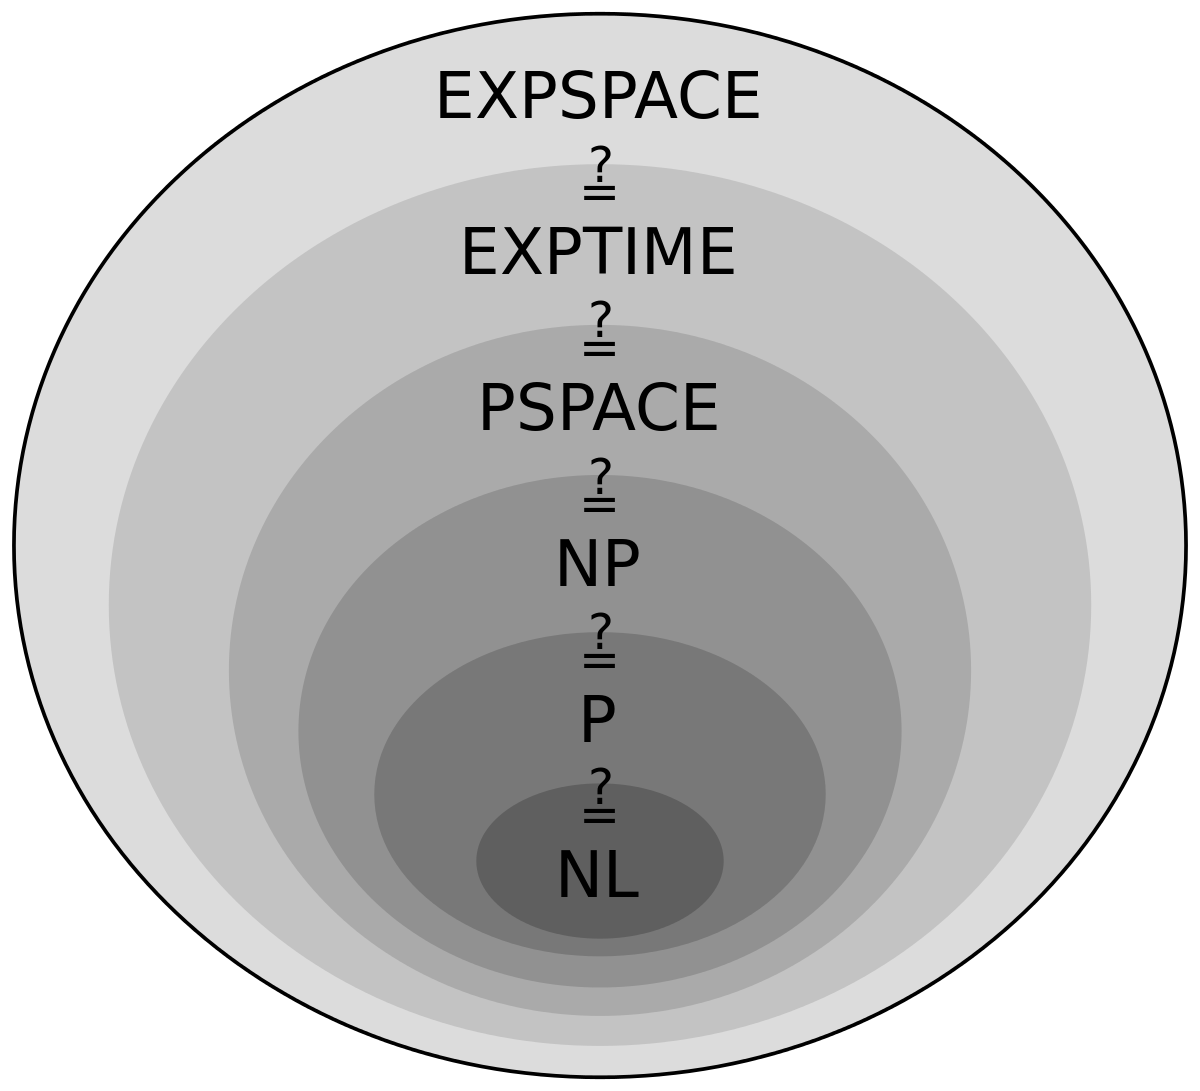
\includegraphics[scale=0.15]{images/classes.png}
\end{center}
\caption{Complexity classes \cite{classesPic}}
\end{figure}

Usually the complexity depends on the input size. With the asymptotic complexity, classes are build, which are the complexity classes. \cite{GTI}


\subsection*{Summary:}

\textbf{Parameters of complexity classes:} \cite{CC, book}

\begin{itemize}
\item \textbf{Model of computation:} \\
here: multistring Turing Machine
\item \textbf{Mode of computation:} \\
for example: deterministic or non-deterministic (deterministic: the computer will always produce the same output for a given input while going through the same states, non-deterministic: can show different behaviors for the same input)
\item \textbf{Resources:} \\ 
something \textit{expensive} that the machine uses up, for example: time or space
\item \textbf{Restrictions/Bound:} \\ 
for example: upper bound, lower bound as a function $f: \mathbb{N} \rightarrow \mathbb{N}$
\end{itemize}

\textbf{Definition of complexity classes:} \cite{book} \\
The complexity class is the set of all languages which are decided by a Turing Mashine $M$ that is operating in the defined mode and for any input $x$, $M$ uses at most $f(|x|)$ units of the defined resource.

\newpage
\textbf{Definition proper complexity function:} \cite{book, CC, GTI}
\begin{itemize}
\item $f: \mathbb{N} \rightarrow \mathbb{N}$
\item $\forall n \in \mathbb{N} \ f(n+1) >= f(n) $ ($f$ is non-decreasing)
\item It exists a multistring Turing Machine $M$ that fullfills the following conditions with an input of size $n$:
\begin{itemize}
\item $M$ halts after $O(n + f(n))$ steps (runs in time $O(n + f(n))$)
\item $M$ uses $O(f(n))$ space
\item $M$ maps $1^n$ to $1^{f(n)}$
\end{itemize}
\end{itemize}

Examples of proper functions: \cite{book} 
\begin{align*}
\ & f(x) = \log n^2 \\
\ & f(x) = n \log n \\
\ & f(x) = n^2 \\
\ & f(x) = n^3 +3n \\
\ & f(x) = 2^n \\
\ & f(x) = \sqrt{n} \\
\ & f(x) = n!
\end{align*}

If the function $f$ and $g$ are proper, $f+g$, $f \cdot g$ and $2^g$ are proper, too.

% TODO: komische potenz/blank sache?
\ \\
\textbf{Definition precise Turing Machine:} \cite{book, CC} \\
A multistring Turing Machine $M$ is called a precise Turing Machine, if there are functions $f$ and $g$ such that, for every input $x$ of length $n$, $M$ stops after exactly $f(n)$ steps with exactly $g(n)$ blanks on strings $2, . . . , k$.

\ \\
If $M$ is a precise Turing Machine and $f$ is a proper complexity functon such that, $M$ decides a language in $f(n)$, then there exists a precise Turing Machine $M'$ of the same type as $M$ which decides the same language in $O(f(n))$.


\ \\
\textbf{Complexity classes:} \cite{book, CC} \\

\begin{tabular}{l|l}
Class name & Description \\
\hline
TIME($f$) & deterministic time \\
SPACE($f$) & deterministic space \\
NTIME($f$) & non-deterministic time \\
NSPACE($f$) & non-deterministic space \\
\end{tabular}
\ \\ \\
($f$ is a proper complexity function) 

\ \\
Sometimes $f$ is not a particular function but a family of function which are parametrized by an integer $k>=0$. 
\ \\ \\
\begin{tabular}{lll}
Class & Function & Description \\
\hline
P & $\bigcup_{k >= 0} $TIME$(n^k)$ & Polynomial time \\
NP&$\bigcup_{k >= 0} $NTIME$(n^k)$ & Non-deterministic polynomial time \\
  EXP & $\bigcup_{k >= 0} $TIME$(2^{n^k})$ & Exponential time \\
   \hline
   L & SPACE$\log n$ & Logarithmic space \\
    NL &  NSPACE$(\log n)$ & Non-deterministic logarithmic space \\
     PSPACE & $\bigcup_{k >= 0} $SPACE$(n^k)$ & Polynomial space \\
      NPSPACE & $\bigcup_{k >= 0} $NSPACE$(n^k)$ & Non-deterministic polynomial space\\
      \hline
\end{tabular}


\newpage
\textbf{Complement classes:} \cite{book, CC} \\

For a string that is part of a language, one \textit{yes} input needs to be found. For a string to be not part of a lanugage, all the paths must be a \textit{no}.
The complement of a language $L \subseteq \Sigma^*$ is the set of all valid inputs that do not belong to $L$. It is denoted as $\bar{L}$ with $\bar{L} = \Sigma^* - L$.
This can be extended to decision problems. The complement of a decision problem $A$ is called $A$ COMPLEMENT.
The \textit{yes} and \textit{no} answers on an Turing Machine can be switched to solve the complement problems.
\ \\
\\
The complement of a complexity class $C$, the class of all the complements is denoded as $coC$. The deterministic classes are closed under complement, for examlpe $coP = P$. That does not cound for non-deterministic classes.


%------------------------------------------------------------------



\section*{Hierarchy problem}



\newpage

\printbibliography




\end{document}